\documentclass[12pt,a4paper]{article}
\usepackage[polish]{babel}
\usepackage[T1]{fontenc}
\usepackage[utf8x]{inputenc}
\usepackage{hyperref}
\usepackage{url}
\usepackage[]{algorithm2e}
\usepackage{listings}
\usepackage{graphicx}
\usepackage{color}
\usepackage{listings}
\usepackage{mathtools}

\lstloadlanguages{% Check Dokumentation for further languages ...
	C,
	C++,
	csh,
	Java
}

\definecolor{red}{rgb}{0.6,0,0} % for strings
\definecolor{blue}{rgb}{0,0,0.6}
\definecolor{green}{rgb}{0,0.8,0}
\definecolor{cyan}{rgb}{0.0,0.6,0.6}

\lstset{
	language=csh,
	basicstyle=\footnotesize\ttfamily,
	numbers=left,
	numberstyle=\tiny,
	numbersep=5pt,
	tabsize=2,
	extendedchars=true,
	breaklines=true,
	frame=b,
	stringstyle=\color{blue}\ttfamily,
	showspaces=false,
	showtabs=false,
	xleftmargin=17pt,
	framexleftmargin=17pt,
	framexrightmargin=5pt,
	framexbottommargin=4pt,
	commentstyle=\color{green},
	morecomment=[l]{//}, %use comment-line-style!
	morecomment=[s]{/*}{*/}, %for multiline comments
	showstringspaces=false,
	morekeywords={ abstract, event, new, struct,
		as, explicit, null, switch,
		base, extern, object, this,
		bool, false, operator, throw,
		break, finally, out, true,
		byte, fixed, override, try,
		case, float, params, typeof,
		catch, for, private, uint,
		char, foreach, protected, ulong,
		checked, goto, public, unchecked,
		class, if, readonly, unsafe,
		const, implicit, ref, ushort,
		continue, in, return, using,
		decimal, int, sbyte, virtual,
		default, interface, sealed, volatile,
		delegate, internal, short, void,
		do, is, sizeof, while,
		double, lock, stackalloc,
		else, long, static,
		enum, namespace, string},
	keywordstyle=\color{cyan},
	identifierstyle=\color{red},
}
\usepackage{caption}
\DeclareCaptionFont{white}{\color{white}}
\DeclareCaptionFormat{listing}{\colorbox{blue}{\parbox{\textwidth}{\hspace{15pt}#1#2#3}}}
\captionsetup[lstlisting]{format=listing,labelfont=white,textfont=white, singlelinecheck=false, margin=0pt, font={bf,footnotesize}}


\addtolength{\hoffset}{-1.5cm}
\addtolength{\marginparwidth}{-1.5cm}
\addtolength{\textwidth}{3cm}
\addtolength{\voffset}{-1cm}
\addtolength{\textheight}{2.5cm}
\setlength{\topmargin}{0cm}
\setlength{\headheight}{0cm}

\begin{document}
	
	\title{Systemy sztucznej inteligencji\\\small{dokumentacja projektu DigitRecognizer}}
	\author{
	Jambor Daniel\\
	Grupa 2D
	\and
	Kozieł Wojtek\\
	Grupa 2D
	\and
	Matula Kamil\\
	Grupa 2D}

	\date{\today}

	\maketitle
	\newpage
	\section*{Część I}
	\subsection*{Opis programu <<JAK DLA MNIE TO STYKNIE - ILE MOŻNA PISAĆ O TAK PROSTEJ RZECZY>>}
	Program DigitRecognizer służy do rozpoznawania ręcznie napisanych  działań i wyświetlanie ich wyniku. Użytkownik pisze na specjalnym polu liczby całkowite oraz jeden z czterech zaimplementowanych wyrażeń arytmetycznych (dodawanie, odejmowanie, dzielenie i mnożenie), a program wyświetla końcowy wynik podanego wcześniej działania. Program korzysta z bazy danych 'MNIST', która składa się łącznie z 70 000 ręcznie napisanych cyfr oraz z autorskiej bazy danych oznaczeń matematycznych.
	
	
	
	
	
	\subsection*{Instrukcja obsługi <<MOŻNA COŚ DOPISAĆ>>}
	Aby uruchomić program, należy uruchomić plik \textit{DigitRecognizer.exe}. Do prawidłowego działania aplikacji wymagany jest plik \textit{weights.txt}, który znajduje się w tym samym folderze co plik \textit{DigitRecognizer.exe}. Jeśli plik nie istnieje, należy pobrać program jeszcze raz. Po uruchomieniu programu, użytkownik zobaczy:
	\begin{itemize}
	\item Białe pole, po którym użytkownik może pisać równania.
	\item Pole tekstowe, gdzie będą wyświetlane wszystkie komunikaty odnośnie działania programu.
	\item Przycisk 'Uruchom sieć neuronową' - jest on jedynym dostępnym przyciskiem po uruchomieniu programu - tworzy on sieć neuronową i wczytuje wcześniej wyuczone wagi.
	\item Przycisk 'Wyczyść' - przycisk który czyści zawartość białego pola.
	\item Przycisk 'Oblicz' - przycisk który pobiera narysowane przez użytkownika działanie i oblicza wynik.
	\end{itemize}
	Aby dostać wynik, użytkownik musi narysować na białym polu równanie. W razie pomyłki może nacisnąć przycisk 'Wyczyść', aby zacząć jeszcze raz. Po narysowaniu równania wystarczy wcisnąć przycisk 'Oblicz', po czym w polu tekstowym pojawi się wynik równania.

	\subsection*{Dodatkowe informacje <<NIE MAM POJĘCIA CO TUTAJ MOŻNA DAĆ ;-;>>}
	Wymagania itd. 
	\newpage
	\section*{Część II}
	\subsection*{Opis działania} 
	Tutaj uwzględniamy część matematyczną. Opisujemy całą teorię np.:
	dla zadania związanego z sieciami neuronowymi - opisujemy całą budowę, algorytm uczenia i wszystkie wzory. Dla zadania związanego z kombinatoryką opisujemy całą teorię kombinatoryczną potrzebną do zrozumienia zadania (mile widziany przykład obliczeniowy).
	
	
	
	\subsection*{Algorytm}
	Tutaj opisujemy rozwiązanie zadania. Dla przedmiotu programowanie będzie to wykorzystanie matematyki z poprzedniego zadania itd. Dla SSI będzie to ogólne działanie przetwarzania danych w oparciu o modele matematyczne z poprzedniego zadania. 
	
	
	Pseudokod tworzymy w \LaTeX. Przykład:\\
	\begin{algorithm}[H]
		\KwData{Dane wejściowe liczba $k$}
		\KwResult{Brak }
		$i:=0$\;
		\While{$i<k$}{
			Drukuj na ekran liczbę $i$\;
			\eIf{$i\%2==0$}{
				Wydrukj informację, że liczba $i$ jest liczbą parzystą\;
			}{
				Wydrukj informację, że liczba $i$ nie jest liczbą parzystą\;
			}
		}
		\caption{Algorytm drukowania informacji o liczbie parzystej/nieprarzystej.}
	\end{algorithm}

	\subsection*{Bazy danych}
	Nauka sieci neuronowej wykorzystywała dwie bazy danych:
	\subsubsection*{MNIST}
	\textbf{THE MNIST DATABASE of handwritten digits} - baza danych skłądająca się z 60 000 próbek treningowych oraz 10 000 próbek walidacyjnych. Dane są przechowywane w formacie \textit{.idx3-ubyte} (w przypadku samych obrazków) oraz \textit{.idx1-ubyte} (w przypadku etykiet). Pliki składają się z wartościu typu ubyte i 32 bit integer. W przypadku plików przechowujących grafiki, pierwsze cztery wartości przechowują:
	\begin{itemize}
	\item 'Magic number' - liczba kontrolna
	\item Liczba zdjęć
	\item Szerokość jednego zdjęcia
	\item Wysokość jednego zdjęcia
	\item Kolejne pixele zdjęć. Pixele te przyjmują wartości od 0 (które reprezentuje kolor biały) do 255 (reprezentacja koloru czarnego)
	\end{itemize}
	
	Pliki przechowujące etykiety zbudowane są na podobnej zasadzie:
	\begin{itemize}
	\item 'Magic number' - liczba kontrolna
	\item Liczba etykiet
	\item Kolejne etykiety
	\end{itemize}
	
	Wczytywanie bazy danych polega na wczytaniu pierwszych czterech wartości z pliku zawierającego zdjęcia oraz pierwszych dwóch z pliku zawierająceego etykiety. Następnie do tablicy dwuwymiarowej wczytywane jest 784 pixeli (28 x 28), a do drugiego wymiaru odpowiadająca zdjęciu etykieta (dla jedynki będzie to 1 itp.). Takie dane są już gotowe do przesłania ich do sieci, jednak etykiety zostały przebudowane na potrzeby projektu.
	
	\subsubsection*{Baza oznaczeń matematycznych}
	Baza oznaczeń matematycznych została zrobiona na potrzeby projektu. Baza opiera się na plikach .png, które zawierają zestawy każdego znaku:
	\begin{center}
	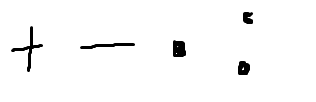
\includegraphics[scale=1]{dane1.png} 
	\end{center}	 
	Jeden plik zawiera 50 takich zestawów umieszczonych w jednym wierszu. Łącznie baza danych składa się z 600 znaków, z czego 10\%  jest traktowana jako część walidacyjna. Za pomocą napisanego algorytmu, plik jest dzielony na 200 osobnych obrazków, których pixele są zapisywane w tablicy tak samo jak w przypadku bazy danych MNIST. Z racji tego, że możliwe są tylko cztery etykiety, dodawane one są naprzemiennie, gdyż kolejność oznaczeń jest taka sama(plus, minus, mnożenie, dzielenie). 
	\subsection*{Implementacja}
	Opis, zasada i działanie programu ze względu na podział na pliki, nastepnie	funkcje programu wraz ze szczegółowym opisem działania (np.: formie pseudokodu, czy odniesienia do równania)
	\begin{lstlisting}
	Tutaj wklejamy fragment kodu, ktory chcemy opisac 
	(bez polskich znakow).
	\end{lstlisting}
	\subsection*{Testy}
	Tutaj powinna pojawić się analiza uzyskanych wyników oraz wykresy/pomiary.
	
	\subsection*{Eksperymenty}
	Sekcję używamy gdy porównywaliśmy dwa lub więcej algorytmów, albo wykonywaliśmy jakies pomiery.
	
	Warto dodać jakies wykresy jako obraz, albo tabele z wynikami. 
	
	Wszyskie wyniki powinny być opisane/poddane komentarzowi i poddane analizie statystycznej.
	\newpage
	\section*{Pełen kod aplikacji}
\begin{lstlisting}
Tutaj wklejamy pelen kod. 
\end{lstlisting}
\end{document}
